\documentclass{article}
  
\title{4site Debugging}
\author{Patrick Daley}

\usepackage{graphicx}

\addtolength{\oddsidemargin}{-.875in}
\addtolength{\evensidemargin}{-.875in}
\addtolength{\textwidth}{1.75in}
\addtolength{\topmargin}{-1.075in}
\addtolength{\textheight}{1.75in}
	
\begin{document}
	
\maketitle
	
This documents summarizes the debugging process of the density of states (DOS) for the Anderson Hubbard 4 site code with on site interactions. The sections are in the order in which each of the simplified simulations were tested. The code file name is main.f90 and used the module in routines.f90.

\subsection*{Atomic Limit with No-Interacting}

A simulation was run with the hoping potential (t) set to zero as well as the on site interactions (U) also set to zero. We were expecting the DOS to be a rectangular shape with one edge starting at -W/2 (W is the disorder strength) and ending at W/2. This was expected because the contributions should occur at the same energies as the site potentials which were chosen from a uniform distribution bounded between -W/2 and W/2. The DOS outputted from the simulation however had a large zero bias anomaly. To find the error we printed the matrices to data files to view them. Upon inspection there were non zero off diagonal terms even though there should be none. What was happening is that even though the matrices were being set to zero in the same line as they were being declared when these declarations were done multiple times (which they were since they were in a loop) and subsequent iterations they were no longer zero. This was solved by setting all the variable to zero again in the body of the code instead of in the declaration statements. The final DOS for this limit is figure 1.

\begin{center}
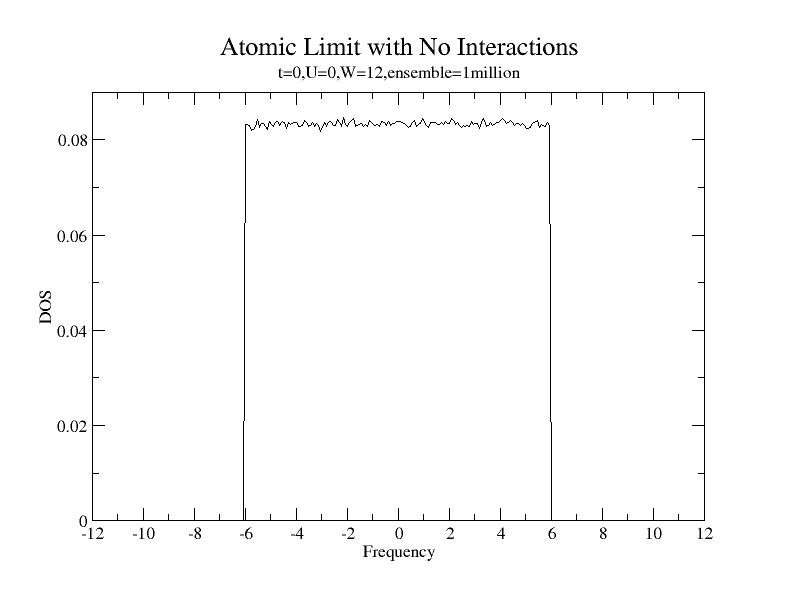
\includegraphics [width=10cm]{dos_t0u0w12.jpg} \\
Figure 1: Graph of the DOS for the atomic limit with no on-site interactions. 
\end{center}
\smallskip
The error initially  was thought to be due to rounding errors since the matrices we big (largest was 36x36). The rounding would cause states that normally should have identical energy to be slightly off creating this anomaly. This was found to not be the case after writing another program that solved similar matrices of the same size which was found to have no appreciable rounding errors.

\subsection*{Atomic Limit with Interactions}

The same simulation as before was run but this time the on site interactions were not set to zero (U/=0). The DOS was expected to still have a rectangular shape. The DOS that was outputted from the program however did not have straight lines on the edges of the rectangles and were instead tapered and had contributions to the DOS at values that were above the allowed range. To find the error the code was modified so that when a contribution was made to the DOS at a value outside the allowed range it would print all the ground state and the site potentials as well as the ground state eigenvector. The program was run multiple times and it was noticed that the illegal contributions would only occur when it was a specific ground state. The photo emission spectrum (PES) and inverse photo emission spectrum (IPES) lookup tables were check for these ground states and the errors were found. The graph of the DOS looked as it should again and the illegal contributions stopped. The final DOS for this limit is figure 2.

\begin{center}
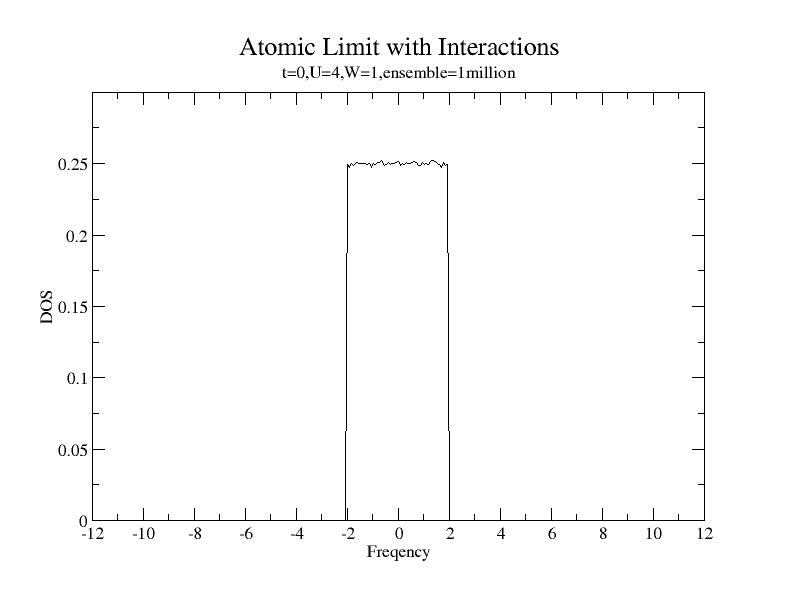
\includegraphics [width=10cm]{dos_t0u4w12.jpg} \\
Figure 2: Graph of the DOS for the atomic limit with on-site interactions. 
\end{center}
\smallskip

\subsection*{Non Atomic Limit with no Interactions}

A simulation was run for t/=0 and U=0. The DOS could be calculated using another code that was already being used to find the DOS for the non interacting case. The other code would simply solved the single particle hamiltonians eigenvalues and make contributions to the DOS at those values. The two DOS were compared by seeding the random generator that is used to chose the site potentials with the same value. The graphs could also be compared to results published by Johri and Bhatt in a recent paper about the non interacting case.

The two DOSs was very different and there was a zero bias anomaly and asymmetries in the DOS outputted by our program. The DOS had almost no contributions above a certain energy in published paper however ours had many. A portion of code was added that would print out the contribution energies as well as the single particle eigenstates (the values the contributions should be occurring at). There was a large difference between these values. The values were all consistently off and would get farther off as the value of t was increased. This lead us to believe the errors would due to mistakes in the hamiltonians. The hamiltonians were all recalculating by hand and some errors were found. Once these errors were fixed the DOS's zero bias anomaly diminished but was still there.

Since the code was almost identical to that of the 2site code which had already been validated all the elements that were different between the two were checked. The hamiltonians were initially calculated by hand and recorded in an excel file. To ensure the matrices had been entered properly into the code another program (compare.f90) was written to compare the matrices in the code and the excel files. The excel files were exported as .csv files and the scripting language "sed" was used to change the commas to semi colon so that fortran could read it. The program took any two files that contained matrices and compared them and printed out each matrix and the location of any differences. This found a few mistakes. The asymmetry and the zero bias anomaly were almost completely gone.

To check if the IPES and PES lookup tables had errors another program was written (trans.f90). This program would create a ground state vector that was any state and would apply the IPES and PES matrices to it and print the states it would transition too. To speed up the process the a extra portion of code was added that would loop over all states and print out error messages if there was not transitions to 8 states (there must always be 8 transitions). This allowed the problematic states to be quickly found and then individually probed and fixed. After fixing these two areas the DOS matched perfectly the results of the separate non-interacting program as well as the published results by Johri and Bhatt. The final DOS for this limit is figure 3.

\begin{center}
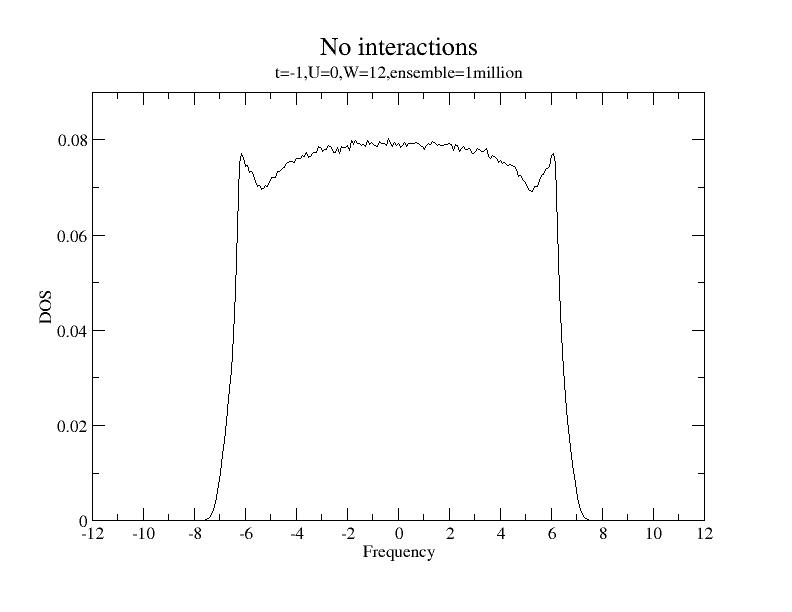
\includegraphics [width=10cm]{dos_t-1u0w12.jpg} \\
Figure 3: Graph of the DOS for the non interacting case.
\end{center}
\smallskip
The program is fully validated and functional at this time.
\end{document}